\chapter{NVARs in Practice}\label{ch:nvar-application}

In this chapter, I resolve the practical questions raised in
\cref{ch:nvar}, and demonstrate that NVARs are capable of solving
traditional RC problems well with very few taps, simple
nonlinearities, and very little training data. Using the example
systems from \cref{ch:systems}, I use NVARs to perform state
inference and forecasting on the Lorenz '63 system, forecasting on the
double-scroll circuit, and forecasting on the Mackey-Glass time-delay
system.

The work presented in this chapter is the result of a
collaboration with Daniel~J.~Gauthier, Erik~Bollt, and Wendson~A.S.~Barbosa~\cite{gauthier2021}. My contribution involves the initial
implementation and exploration of the NVAR method, discussion during
the development of the Lorenz '63 results, as well as the
implementation of the Lorenz return map, double-scroll forecasting,
and Mackey-Glass forecasting.

\section{State Inference with Lorenz '63}

For this inference task, I provide an NVAR with the $x$ and $y$
components of the Lorenz '63 system, and train it to infer the third
$z$ variable. Inference tasks like this are useful in situations where
some variables of a system are easily measurable, while the rest are
only measurable with great care or expense. For example, a mechanical
engine can be outfitted at great expense with a large array of
internal temperature and pressure sensors, and an NVAR can be trained
to infer these variables from easily-accessible external sensors. Once
trained, the NVAR can now be reused on engines manufactured without
the expensive internal instrumentation.

For this task, I use an integration time-step of $\Delta t = 0.05$. To
build an NVAR, I must choose the tap delays $\tau_i$, the
nonlinearity $\bm{g}_\text{n}$, and ridge parameter $\alpha$. Takens'
embedding theorem~\cite{takens1981} provides guidance on the expected
number of taps: as the dimension of the Lorenz attractor is slightly
larger than $2$, I choose to use $4$ equally spaced taps $\tau_0 =
0$, $\tau_1 = 5$, $\tau_2 = 10$, and $\tau_3 = 15$. These taps are
spaced to equally cover roughly one Lyapunov period, with the last tap
at time $\tau_3 \Delta t = 0.75$.

For the nonlinearity $\bm{g}_\text{n}$, I use a slightly modified
version of the quadratic output introduced in
\cref{eq:quadratic-nvar}. This $\bm{g}_\text{n}$ includes a constant
term, all linear terms of the tap vector $\bm{v}$, and all quadratic
terms of the tap vector $\bm{v}$. That is,
\begin{equation}
  \label{eq:quadratic-nvar-const}
  \bm{g}_\text{n}(\bm{v}) = 1 \oplus \bm{v} \oplus \ceil{\bm{v} \otimes \bm{v}}.
\end{equation}
The addition of a constant term allows the trained linear
$W_\text{out}$ to fit a constant offset, which is useful here as the
$z$ component is always positive, even when both $x$ and $y$ are zero.

For this task, with $q = 4$ taps and $d = 2$ input dimensions, $x$ and $y$, the
output of $\bm{g}_\text{n}$ has $1 + 8 + 36 = 45$ components, and the linear
output matrix $W_\text{out}$ has dimension $1 \times 45$.

\begin{figure}
  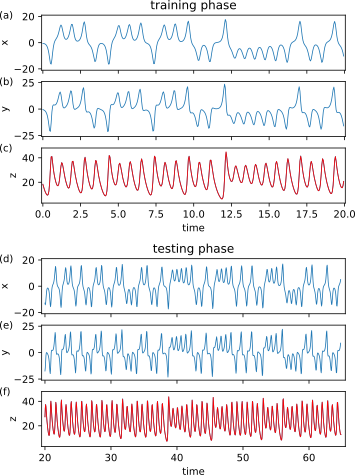
\includegraphics{figures/nvar-infer-lorenz}
  \caption{(a) -- (c) The Lorenz '63 system (blue) during the NVAR
    training. After the NVAR is trained, it is re-used on the
    training signal to produce the training output (c, red). (d) --
    (f) The Lorenz '63 system during NVAR testing, with the NVAR
    output. In both cases, the NVAR output (red) lies directly on top
    of the true Lorenz signal (blue).}
  \label{fig:nvar-infer-lorenz}
\end{figure}

I train this NVAR on $10$ different examples of the Lorenz '63
system, using $x$ and $y$ as the example input and $z$ as the example
output. Each training example is $20$ time units. I then evaluate
the NVAR for $45$ time units to produce a NRMSE $\epsilon$ as in
\cref{eq:nrmse}, and then average these errors over all $10$
trials. During evaluation, the NVAR has access to only $x$ and $z$,
and must produce an estimate of $z$. I then adjust $\alpha$ manually
to minimize this error. This whole process, training the NVAR $10$
different times and evaluating the error, takes only a few seconds on
a modern computer even with a poorly-optimized implementation.

I find this NVAR has a NRMSE of $1.75\mp0.3\times10^{-2}$ on this
inference task, using the ridge parameter $\alpha = 0.05$. An example
of the NVAR during a single training and testing trial is shown in
\cref{fig:nvar-infer-lorenz}. The trained NVAR shows good agreement in
the $z$ component during both the training phase (c) and the testing
phase (f); in fact, the agreement is so good that when the NVAR signal is
drawn on top of the true Lorenz signal, the true signal is not visible
underneath.

\subsection{Output Weights}\label{sec:nvar-infer-weights}

The output weights $W_\text{out}$ from a single trial, visualized in
\cref{fig:nvar-infer-lorenz-wout}, have two notable features. First,
the largest trained weight by far corresponds to the $1$ term in
$\bm{g}_\text{n}$. This accounts for the fact that $z$ is always
positive, and justifies the inclusion of the constant term in
$\bm{g}_\text{n}$.

\begin{figure}
  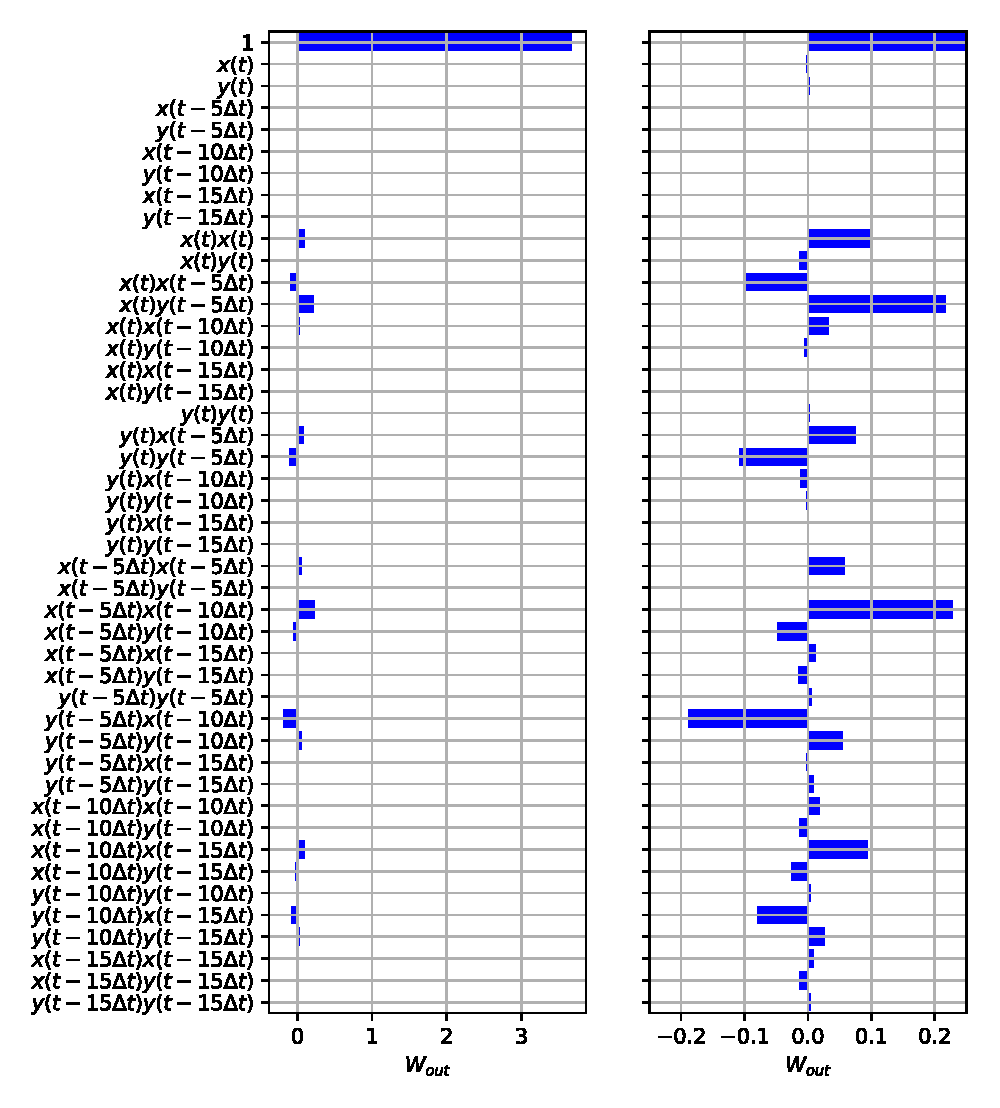
\includegraphics[width=\textwidth]{figures/nvar-infer-lorenz-wout}
  \caption{Weights in the matrix $W_\text{out}$ (left) for the NVAR
    trained for Lorenz system forecasting. On the right, a magnified
    view of the same. The largest component is the constant offset, to
    account for the fact that the $z$ component of the Lorenz system
    is positive, even when both $x$ and $y$ are zero. Also note that
    the linear terms in $x$ and $y$ have weights near zero. As the
    Lorenz system has a $(x, y) \rightarrow (-x, -y)$ symmetry, the
    NVAR must have zero weights attached to these terms to respect
    that symmetry.}
  \label{fig:nvar-infer-lorenz-wout}
\end{figure}

Second, the weights of all the linear terms in $x$ and $y$ are all
near zero. This reflects the $(x, y) \rightarrow (-x, -y)$ symmetry of
the Lorenz system. Since the NVAR input $\bm{u}(t)$ is just these $x$
and $y$ terms, in order to respect this symmetry the NVAR must predict
the same $z(t)$ for both $\bm{u}(t)$ and $-\bm{u}(t)$. This is only
possible if the linear terms in $x$ and $y$ have zero coefficients.

In general, an NVAR does not need to respect the symmetries of the
entire underlying system: if the NVAR is trained on only a small part
of the input system's phase space, it does not need to respect
symmetries outside that space to perform well within that space. Here,
however, the NVAR training input $\bm{u}_\text{train}(t)$ overlaps
with its symmetric counterpart $-\bm{u}_\text{train}(t)$, and so learning
the example input necessarily means learning the symmetry.

Later, in \cref{sec:nvar-mackey-glass}, I will investigate a task
where the example input does not overlap with its symmetric
counterpart, and demonstrate that the NVAR will learn weights that do
not agree with this symmetry.

\section{Forecasting Lorenz '63}

For this task, I use an NVAR in forecasting mode to do system
forecasting for the Lorenz '63 system. That is, I train the NVAR to
use all three state variables $x$, $y$, and $z$ to perform
next-step-ahead prediction of the Lorenz system in
\cref{eq:lorenz}. Unlike for the inference task, the NVAR has no
external driving input and runs autonomously once it is in forecast
mode. In analogy to other discrete-time integration algorithms, the
choice of time step $\Delta t$ has a stronger effect on forecasting
than inference. Too small a time step is wasted effort, and too large
risks inaccuracy. Here, I use a time step of $\Delta t = 0.025$, which
results in about $40$ steps per Lyapunov period.

For this forecasting task, I use only $2$ taps, $\tau_0 = 0$ and
$\tau_1 = 1$. That is, the NVAR has access to the two previous time
steps, and I find this is enough for the forecasting task.  I use the
quadratic nonlinearity with constant term described in
\cref{eq:quadratic-nvar-const}. With $q = 2$ taps and $d = 3$ input dimensions,
the nonlinear output of $\bm{g}_\text{n}$ has $1 + 6 + 21 = 28$
components, and so $W_\text{out}$ has dimension $3 \times 28$.

Again, I train this NVAR on $10$ different examples of the Lorenz '63
system, each time training on $10$ time units. I then evaluate the
NVAR by performing an autonomous forecast for one Lyapunov period to
calculate a NRMSE $\epsilon_1$, as in \cref{eq:nrmse}, and then
average this over the $10$ trials to produce $\tilde{\epsilon}$ in
\cref{eq:nrmse-avg}.

\begin{figure}
  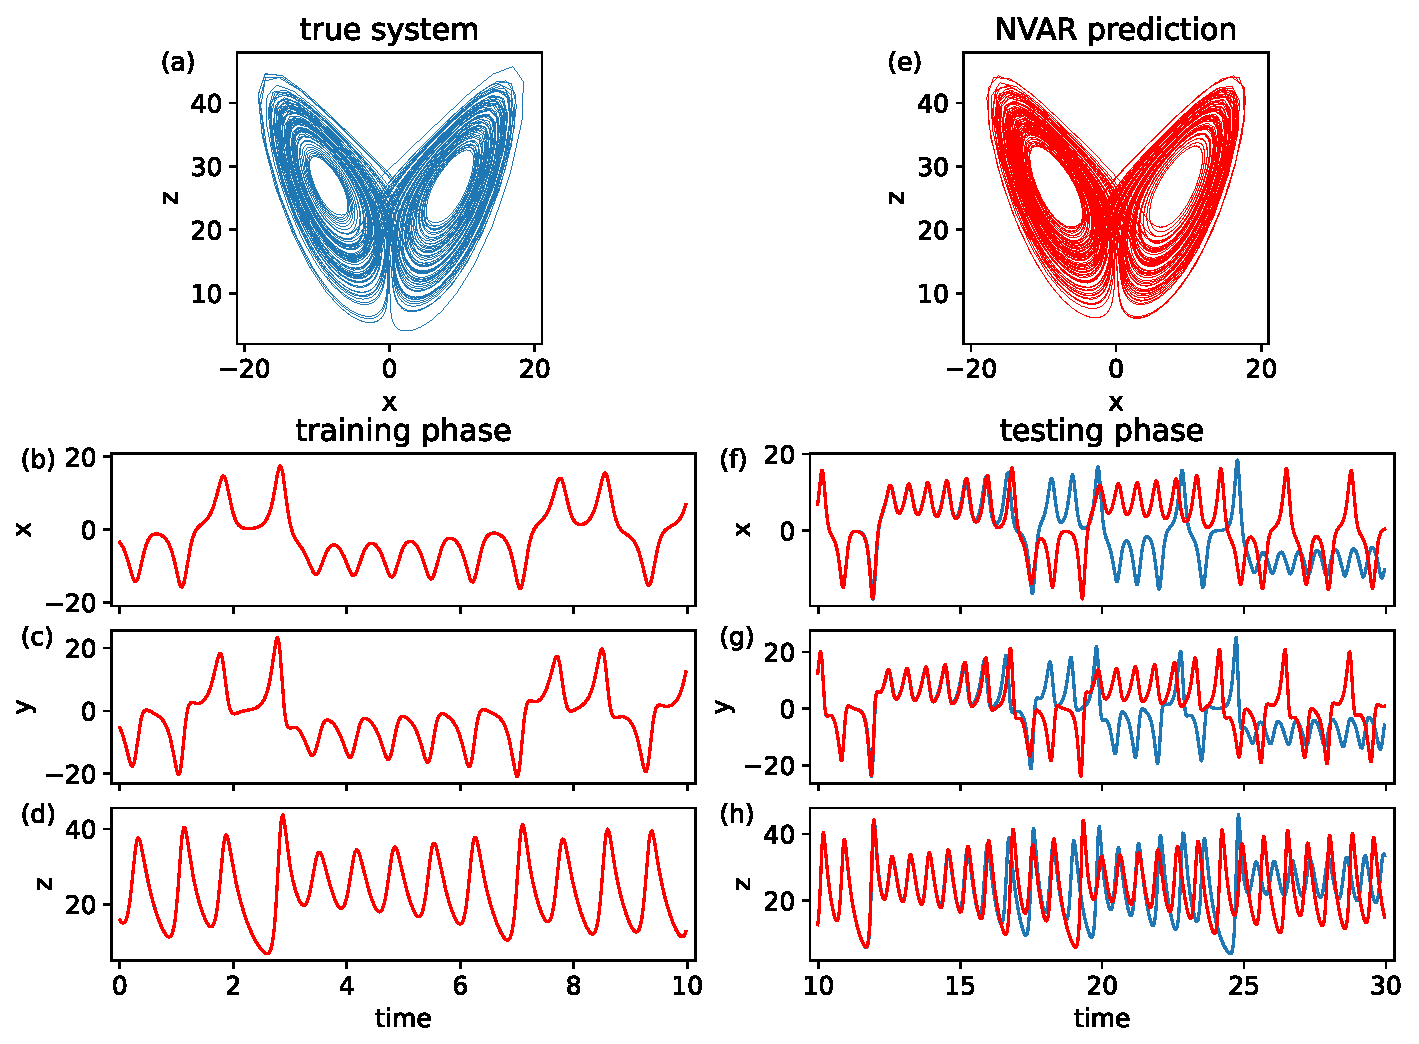
\includegraphics[width=\textwidth]{figures/nvar-predict-lorenz}
  \caption{The true Lorenz attractor (a) and NVAR predicted attractor
    (e) for a single training trial. (b)~--~(d) True Lorenz system
    (blue) during training overlaid with NVAR output (red) calculated
    after training is complete. (f)~--~(h) True (blue) and NVAR
    forecasted output (red). The NVAR shows good agreement with the
    true system as far as $5$ Lyapunov periods in to the autonomous
    forecast.}
  \label{fig:nvar-predict-lorenz}
\end{figure}

The performance of this NVAR during a single training trial is shown
in \cref{fig:nvar-predict-lorenz}. A long autonomous forecast from the
NVAR produces an attractor (e) that shows qualitative agreement with
the true Lorenz attractor (a), and produces a NRMSE over one Lyapunov
period of $4.51\pm0.85\times10^{-3}$ using $\alpha =
2.5\times10^{-6}$, about five times better than the ESNs described in
\cref{tab:lowk-lorenz-results}. This NVAR performs better than the
ESNs despite the fact that it is simpler to describe and implement,
does not require lengthy optimization, and trains at least an order of
magnitude faster. The training data used for the NVAR is also very
light: only $10$ time units, corresponding to $400$ points at this
time step, is enough to train the NVAR. During training, the NVAR's
output (b)~--~(d) matches the true signal so well it obscures it, and
during testing, the autonomous forecast (f)~--~(h) only visibly
diverges from the truth after 5 Lyapunov exponents.

\subsection{$z$ Return Map}

The $z$ variable of the Lorenz '63 system has a functional relation
between successive local maxima. This is demonstrated visually by
finding the local maxima $z_i$ of $z$, and then plotting $z_i$ with
respect to $z_{i+1}$ \cite{lorenz1963}. This \emph{return map} neatly
summarizes the long-term behavior of the $z$ variable, and comparing
two such maps provides a quick way to qualitatively compare two
systems. This comparison has been used previously to verify that a
trained RC can replicate the Lorenz '63 dynamics~\cite{pathak2017}.

\begin{figure}
  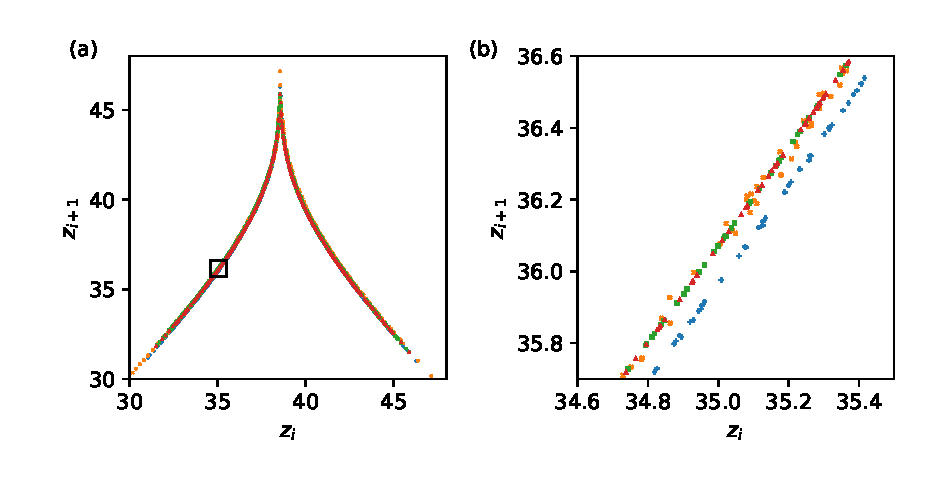
\includegraphics{figures/lorenz-rmap-tol}
  \caption{(a) The $z$ return map of the Lorenz '63 system, integrated
    using various methods. (b) Detail of the region marked in
    (a). Using a relative integration tolerance of $10^{-3}$, the
    Runge-Kutta~3(2) (blue $+$) differs from R-K~5(4) (orange
    $\times$) in both position and spread. Both methods converge after
    sharpening the tolerance to $10^{-5}$ (green square and red
    triangle, respectively).}
  \label{fig:lorenz-rmap-tol}
\end{figure}

In many ways, this comparison is similar to the visual inspection of
the reproduced attractor in \cref{fig:nvar-predict-lorenz}. However,
the return map is a simpler shape and is much more sensitive to error
than the attractor itself, even when comparing two maps by
eye. Indeed, the return map is so sensitive that it depends on the
specific integrator used to find the true Lorenz '63 solution. In
\cref{fig:lorenz-rmap-tol}, I show this return map calculated on a
Lorenz solution produced by four different integrators. All four
methods agree on a large scale, but the zoomed view in (b) reveals
their differences. Using a relative tolerance of $10^{-3}$, the
Runge-Kutta~3(2) method produces a narrow, nearly one-dimensional
return map slightly offset from the much wider return map produced by
Runge-Kutta~5(4). Both algorithms agree after sharpening the tolerance
to $10^{-5}$.  In this chapter, I use the
Runge-Kutta~3(2)~\cite{dormand1980} integrator with $10^{-3}$ relative
tolerance for both the Lorenz '63 and double-scroll systems.

The values of the maxima in the discrete-time solutions for both the
NVAR and Lorenz '63 system depend on the time step $\Delta t$ used for
integration, as the true maximum may be achieved in between the
discrete time steps. To better reproduce the true Lorenz '63 return
map, and to reduce the effect $\Delta t$ has on the NVAR return map,
I interpolate the $z$ solutions by using a degree-$4$ spline. The
local maxima are then found on this interpolated spline~\cite{dierckx1995}.

\begin{figure}
  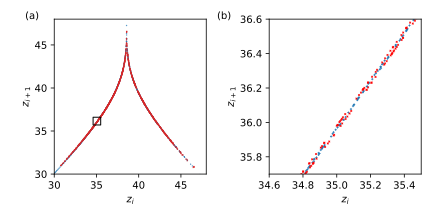
\includegraphics{figures/nvar-lorenz-rmap}
  \caption{(a) The $z$ return map of the Lorenz '63 system (blue $+$)
    overlaid with the $z$ return map of the NVAR forecast (red
    $\times$), trained for $10$ time units. The NVAR reproduces the
    long-term dynamics of the $z$ variable accurately enough at this
    scale that it is difficult to see the true return map
    underneath. (b) Detail of the region marked in (a). At this scale,
    it is possible to see that the NVAR return map is wider than the
    true Lorenz return map, although they lie on top of each
    other. This reproduction can be improved by training the NVAR for
    longer (see \cref{fig:nvar-lorenz-rmap-extra}).}
  \label{fig:nvar-lorenz-rmap}
\end{figure}

\begin{figure}
  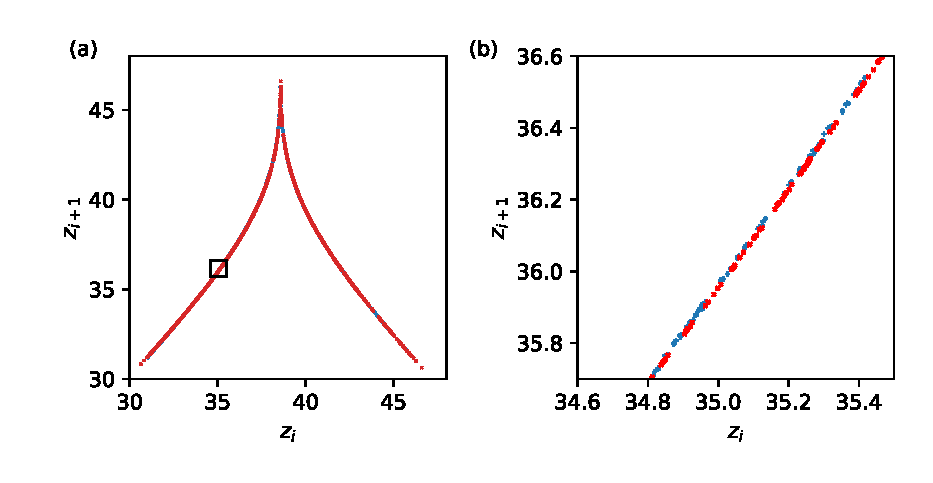
\includegraphics{figures/nvar-lorenz-rmap-extra}
  \caption{(a) The $z$ return map of the Lorenz '63 system (blue $+$)
    overlaid with the $z$ return map of the NVAR forecast (red
    $\times$), trained for $20$ time units. (b) Detail of the
    region marked in (a). With more training time, the NVAR return map
    is narrower and more accurately reproduces the Lorenz return
    map.}
  \label{fig:nvar-lorenz-rmap-extra}
\end{figure}

\Cref{fig:nvar-lorenz-rmap} shows the return maps for both the true
Lorenz system and the NVAR. Qualitatively, there is good agreement
between the two. The NVAR return map almost completely obscures the
true Lorenz return map in (a). Upon close inspection in (b), I see
that the NVAR return map has a width that is wider than that of the
true return map. This can be improved by extending the training time
of the NVAR. The difference between the two return maps is already
small even when the NVAR is trained for only $10$ time units; when
training for $20$ time units, as in \cref{fig:nvar-lorenz-rmap-extra},
the NVAR's predicted return map narrows and lies on top of the true
return map.

As with the attractor comparison, a quantitative measure of return map
similarity would be a strong candidate for replacing the flawed NRMSE
measure.

\subsection{Fixed Points}

For a more quantitative measure of how well the NVAR learns the
dynamics of the Lorenz system, I calculate the fixed points of the
trained NVAR and then find their distance to the true Lorenz fixed
points. By setting the derivatives in \cref{eq:lorenz} to zero, I
find three fixed points of the Lorenz system located at
\begin{align}
  [x, y, z] &= [0, 0, 0], \\
            &= [\pm \sqrt{\beta(\rho - 1)}, \pm \sqrt{\beta(\rho - 1)}, (\rho - 1)].
\end{align}

% fsolve, 'hybr' method, "Powell hybrid method"
% More, Jorge J., Burton S. Garbow, and Kenneth E. Hillstrom. 1980. User Guide for MINPACK-1.
To find the fixed points of the NVAR system, I perform a trial
single-step forecast with a constant past history, and use a
root-finding algorithm to find the specific values of past history
that result in an unchanged forecast. This root-finding algorithm is
used three times, using the three true Lorenz fixed points as initial
guesses.

To allow easy comparison of the accuracy of these fixed points with
other systems, I calculate the distance between this fixed points in
a uniformly scaled space where the Lorenz63 system has unit
variance. For this trained NVAR, the distance from the zero fixed point
is $1.2\pm1.4\times10^{-3}$, and the distances between the predicted
and true positive and negative fixed points are
$11.6\pm3.0\times10^{-4}$ and $7.4\pm1.5\times10^{-4}$, respectively.

The NVAR shows good agreement on the zero fixed point, as the variance
caused by different training windows overlaps with the true
location. The other two fixed points are consistently offset from the
truth. However, in all three cases, the fixed points lie within
approximately $0.1\%$ of the true location, despite the fact that the
training data does not include any of these points.

\subsection{Output Weights}

The particular choice of nonlinearity $\bm{g}_\text{n}$ for this task
completely includes all terms on the right hand side of the Lorenz
system in \cref{eq:lorenz}. That is, the Lorenz system is described by
a polynomial of degree $2$, and the choice of $\bm{g}_\text{n}$ allows
the NVAR to describe \emph{any} polynomial of degree $2$. This raises
a legitimate question: is the NVAR simply performing so well because
it was equipped ahead of time with the perfect tools?

The answer in a general context is no. Just as finite polynomials can
approximate non-polynomial functions arbitrarily well, a continuous
nonlinear dynamical system can be approximated arbitrarily well by a
finite Volterra series~\cite{franz2006}, and NVARs with polynomial
outputs are finite Volterra series with very simple kernels. From this
fact, I expect NVARs with quadratic nonlinearity to be able to
approximate even non-polynomial systems, and so it is not surprising
that it can also approximate quadratic polynomial systems.

\begin{figure}
  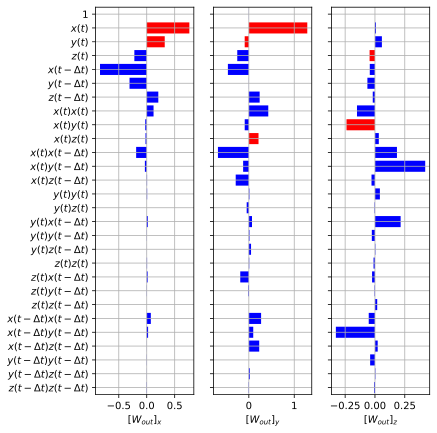
\includegraphics[width=\textwidth]{figures/nvar-predict-lorenz-wout}
  \caption{Weights in the matrix $W_\text{out}$ for the NVAR trained
    for Lorenz system forecasting. Terms that appear directly in the
    Lorenz system (\cref{eq:lorenz}) are in red. There does not appear
    to be any correlation between a large weight in the NVAR output,
    and presence in the Lorenz equations.}
  \label{fig:nvar-predict-lorenz-wout}
\end{figure}

Another way to allay these concerns is to look at other non-polynomial
systems, as in the next few sections. However, even with the Lorenz
system, I see that this is not the case by inspecting the trained
weight matrix $W_\text{out}$ in
\cref{fig:nvar-predict-lorenz-wout}. The terms on the right hand side
of the Lorenz system (marked in red) are present with non-zero weights
in the output matrix, but there are also significant contributions
from other terms, and there does not appear to be a preference for the
NVAR to rely on Lorenz terms only.

From this I derive an interpretation: a trained NVAR is finding the
best possible one-step-ahead integrator it can find, given the example
input and the available terms in $\bm{g}_\text{n}$. When the time step
is large enough, a strictly linear prediction becomes more and more
inaccurate, and so the NVAR relies on the nonlinear and time-delayed
terms to make up the difference.

\section{Forecasting the Double-Scroll Circuit}

For this task, I use an NVAR in forecasting mode to use all
three state variables $V_1$, $V_2$, and $I$ of the double-scroll
circuit described by \cref{eq:dscroll}. I use the same tap
delays $\tau_0 = 0$, $\tau_1 = 1$ as the Lorenz case, but I modify
the choice of nonlinearity.

Unlike the Lorenz system, the double-scroll circuit cannot be
described by a polynomial of degree $2$. Indeed, the double-scroll
equations are odd, and have full inversion symmetry. On top of this,
the double-scroll attractor includes this symmetry; it is identical to
its symmetric partner. As discussed in \cref{sec:nvar-infer-weights},
this drives the contribution of any even terms in $\bm{g}_\text{n}$ to
zero in the trained weight matrix $W_\text{out}$. In light of this, I
use a nonlinear function that includes all linear terms of the tap
vector $\bm{v}$ as well as all terms with degree $3$, but includes no
even terms. That is,
\begin{equation}
  \bm{g}_\text{n}(\bm{v}) = \bm{v} \oplus \ceil{\bm{v} \otimes \bm{v} \otimes \bm{v}}.
\end{equation}
With $q = 2$ taps and $d = 3$ input dimensions, the output of
$\bm{g}_\text{n}$ has $6 + 56 = 62$ components, and so $W_\text{out}$
has dimension $3 \times 62$.

The Lyapunov time of the double-scroll circuit is roughly $10$ times
longer than that of the Lorenz system. To ensure a fair comparison, I
extend the training time of the NVAR from $10$ to $100$ units to keep
the number of Lyapunov times covered by the training similar for both
cases. I also set $\Delta t = 0.25$, to ensure that both the Lorenz
and double-scroll cases use $400$ data points during training.

\begin{figure}
  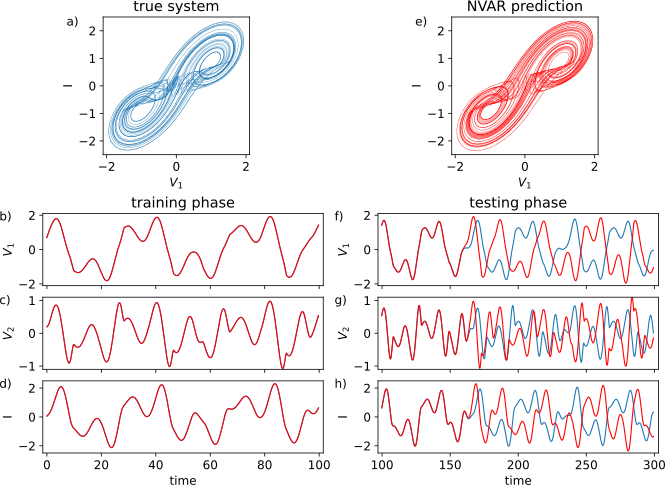
\includegraphics[width=\textwidth]{figures/nvar-predict-dscroll}
  \caption{The true double-scroll attractor (a) and NVAR predicted
    attractor (e) for a single training trial. (b)~--~(d) True
    double-scroll system (blue) during training overlaid with NVAR
    output (red) calculated after training is complete. (f)~--~(h)
    True (blue) and NVAR forecasted output (red). Here, the NVAR
    shows good agreement with the true system as far as $6$ Lyapunov
    periods.}
  \label{fig:nvar-predict-dscroll}
\end{figure}

Other than these modifications, the method for using the NVAR to
forecast the dynamics of this system proceeds exactly as for the Lorenz
system, training the NVAR on $10$ different examples of the
double-scroll circuit and then evaluating the NRMSE for one Lyapunov
period each. The performance of this NVAR during a single training
trial is shown in \cref{fig:nvar-predict-dscroll}.

Once again, a long autonomous forecast (e) shows the NVAR can
reproduce the shape of the double-scroll attractor (a), and over one
Lyapunov period has an NRMSE of $2.15\pm0.63\times10^{-2}$ using
$\alpha = 1.0\times10^{-3}$, about $1.5\times$ better than the ESNs
described in \cref{tab:lowk-resultsplus}. During training (b)~--~(d)
the NVAR matches the system so well the true signal cannot be seen
underneath, and once autonomous forecasting begins in (f)~--~(h), the
NVAR's prediction lies on top of the true system for $6$ Lyapunov
periods.

\subsection{Fixed Points}

Again, I look for the fixed points of this trained NVAR and find
their distance to the true fixed points of the double-scroll circuit,
in a space uniformly scaled so that the double-scroll circuit has unit
variance. Setting the derivatives in \cref{eq:dscroll} to $0$
and solving yields the transcendental equation
\begin{equation}
  0 = \frac{V_1}{R_2}(R_1 - R_2 - R_4) + 2 R_1 I_r \sinh\left(\alpha V_1 \left(1 - \frac{R_4}{R_1}\right)\right).
\end{equation}
For the parameters I use, this yields three solutions for $V_1$. If
$V_1^+$ is the positive solution, this corresponds to three fixed points
at
\begin{align}
  [V_1, V_2, I] &= [0, 0, 0], \\
                &= [V_1^+, \pm V_1^+ R_4 / R_1, \pm V_1^+ / R_1].
\end{align}

Since my choice of $\bm{g}_\text{n}$ has only odd polynomial powers
and no constant term, it is symmetric about the origin and predicts
the zero fixed point exactly. The distance from the true positive
fixed point is $2.7\pm0.3\times10^{-3}$. Due to the inversion
symmetry, the negative fixed point is precisely the same
distance. Although the variance from repeated trials does not overlap
the true fixed points, they do lie within $0.3\%$ of the truth.

This NVAR performs well at short-term forecasting and fixed point
prediction, despite not having access to the infinite number of
polynomial terms in the expansion of the double-scroll equations. This
demonstrates a possible practical approach to NVAR design: keep adding
delay taps and higher polynomial terms to the nonlinear function
$\bm{g}_\text{n}$ until performance is acceptable. However, for NVARs
that require many taps or operate on high-dimensional inputs, this
very quickly leads to an explosion in the number of weights trained in
$W_\text{out}$, and consequently a huge increase in training time. In
the next section, I explore how careful use of tap spacing can
keep the number of taps required low.

\section{Forecasting Mackey-Glass}\label{sec:nvar-mackey-glass}

For this task, I again use an NVAR in forecasting mode, this time
using the single Mackey-Glass state variable $u$ in
\cref{eq:mackey-glass} as input, with $\Delta t = 0.2$. I use the
\texttt{jitcdde} Python package~\cite{ansmann2018} to integrate this
time-delay differential equation. For this system, using two adjacent
taps for the NVAR as in the previous examples is insufficient, as the
Mackey-Glass system behavior depends strongly on both the value of
$u(t)$ as well as $u(t - 17)$. One way to access this value in the
NVAR is to add taps at every time step until they reach $t = 17$,
resulting in $85$ total taps. Even with only a quadratic output, this
requires training a $W_\text{out}$ with dimension $1 \times
3741$. This cost can be avoided by increasing the time step $\Delta
t$, thus reducing the total number of taps, but this solution comes
with the cost of a much more granular prediction.

Another way to access the value at $u(t-17)$ is to use sparse
taps. Here, I use three clusters of two adjacent taps: one cluster at
$\tau_0 = 0$ and $\tau_1 = 1$, one cluster at $\tau_2 = \floor{17 / 2
  \Delta t}$ and $\tau_3 = \tau_2 + 1$, and one cluster at $\tau_4 =
\floor{17 / Delta t}$ and $\tau_5 = \tau_4 + 1$. Here, $\floor{a}$ refers to the integer floor of $a$. This gives the NVAR
access to information at $u(t - 17)$ as well the midpoint $u(t -
17/2)$. I find that adding the tap cluster at the midpoint improves performance
by a factor of $3$, and increases the number of features available to
$W_\text{out}$ to be comparable to the other tasks in this chapter.

The Mackey-Glass system exhibits full inversion symmetry. However,
unlike the double-scroll circuit, the Mackey-Glass system has two
distinct attractors that do not overlap. Any solution on the positive
attractor will remain positive, and never cross over zero to the
negative attractor. Since I am only training the NVAR on a positive
solution to Mackey-Glass, I include even terms in $\bm{g}_\text{n}$. In
fact, I find that including these even terms improves NRMSE
performance. In \cref{sec:nvar-mg-weights}, I demonstrate that the trained NVAR is assigning these terms non-zero weights.

Therefore, I use a nonlinear function
$\bm{g}_\text{n}$ that includes the constant, linear, quadratic, and
cubic terms constructed from the tap vector $\bm{v}$,
\begin{equation}
  \bm{g}_\text{n}(\bm{v}) = 1 \oplus \bm{v} \oplus \ceil{\bm{v} \otimes \bm{v}} \oplus \ceil{\bm{v} \otimes \bm{v} \otimes \bm{v}}.
\end{equation}
With $q = 6$ taps and $d = 1$ input dimension, the output of $\bm{g}_\text{n}$
has $1 + 6 + 21 + 56 = 84$ components, and so $W_\text{out}$ has
dimension $1 \times 84$.

The Lyapunov time of the Mackey-Glass system is roughly $100$ times
longer than that of the Lorenz system. However, I find that a
relatively fine step size $\Delta t = 0.2$ is required for the NVAR to
learn the system, corresponding to $500$ points per Lyapunov period. I train this NVAR for $1000$ time units,
corresponding to $5000$ data points total. Though this is many more
discrete data points, it covers about $10$ Lyapunov times, comparable
to the training time used for the other systems.

This NVAR is much more data hungry than the previous examples,
requiring more training data to produce an acceptable result. This may
be due to the wide tap spacing: values at $u(t - 17)$ are less
correlated to $u(t)$, while $u(t - \Delta t)$ is more correlated, and
so the NVAR needs more data to see every relevant combination of
values at the taps.

\begin{figure}
  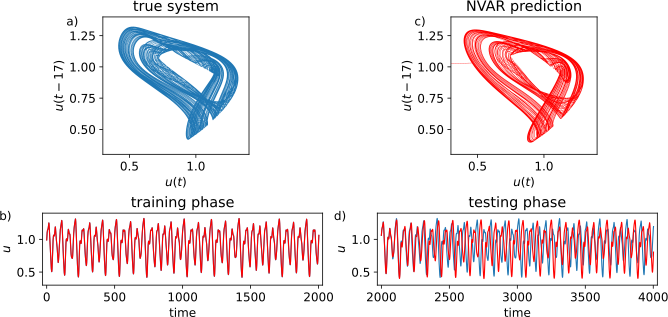
\includegraphics[width=\textwidth]{figures/nvar-predict-mackey-glass}
  \caption{The true Mackey-Glass attractor (a) and NVAR predicted
    attractor (c) for a single training trial. (b) True Mackey-Glass
    system during training overlaid with NVAR output (red) calculated
    after training is complete. (d) True (blue) and NVAR forecasted
    output (red). Here, the NVAR shows good agreement with the true
    system as far as $2$ Lyapunov periods.}
  \label{fig:nvar-predict-mackey-glass}
\end{figure}

Other than these modifications, the methodology for training and
evaluating the NVAR is exactly as for the other two systems. The
performance of this NVAR during a single training trial is shown in
\cref{fig:nvar-predict-mackey-glass}. Over one Lyapunov period, this
NVAR has a NRMSE of $5.77\pm0.42\times10^{-2}$ with $\alpha =
9\times10^{-3}$.

The long autonomous forecast (c) of the NVAR shares important features
with the true attractor (a), most notably the gap between the
bands. However, it does not get some fine details correct, notably the
shape of the heel in the upper-left corner and the overlapping bands
in the middle. This is reflected in the higher NRMSE than the other
tasks. However, as before the NVAR prediction completely obscures the
true system signal during training (b), and once autonomous
forecasting (d) begins the NVAR forecast covers the true system for $2$
Lyapunov periods.

The shape of this heel can be better reproduced by including
higher-order terms in the nonlinear function
$\bm{g}_\text{out}$. However, it is not possible to do this with
monomial terms as I have been doing without dramatically increasing
the training time of $W_\text{out}$. Adding a fourth-order term to $\bm{g}_\text{out}$ increases the number of weights in $W_\text{out}$ by a factor of $3$. This problem becomes even worse on input systems with a dimension higher than $d = 1$.

It may be possible to instead add
nonlinear terms to $\bm{g}_\text{out}$ with an infinite power series,
such as $e^{v_iv_j}$ or $\sinh{v_i}\cosh{v_j}$. This would provide
access to high-order nonlinearity without a corresponding large increase in training
time. This is one important avenue for future research, and this
Mackey-Glass forecasting example demonstrates that cubic terms are not
completely sufficient for accurate forecasts. Nonetheless, the cubic
NVAR used here shows promising performance from a simple model.

\subsection{Fixed Points}

Setting the derivative in \cref{eq:mackey-glass} to $0$ and assuming a
constant past yields three fixed points, located at
\begin{align}
  u &= 0, \\
  u &= \pm \left(\frac{\beta}{\gamma} - 1\right)^{1/n}.
\end{align}
I use these as initial guesses to find the fixed points of the trained NVAR, in a space uniformly scaled so that Mackey-Glass has unit variance.

The distance to the true positive fixed point is
$2.3\pm0.03\times10^{-3}$. The variance from repeated trials does not
overlap the true fixed point, however, it does lie within $0.3\%$ of
the truth.

The NVAR completely fails to predict the $0$ fixed point and the
negative fixed point. This is a consequence of my choice not to
respect the known symmetries of the Mackey-Glass system in favor of
more accurate prediction on the positive attractor. If accuracy on the
non-positive fixed points is desired, the NVAR can be either modified
to respect that symmetry ahead of time, or trained on data from both
the positive and negative attractors.

\subsection{Output Weights}\label{sec:nvar-mg-weights}

The output weights for this task are in
\cref{fig:nvar-predict-mackey-glass-wout}. As expected from the
failure to predict the non-positive fixed points, the NVAR
assigns non-zero weights to those terms (in red) that break the
total inversion symmetry. As the training input does not include any
data from the negative Mackey-Glass attractor, the NVAR has no cause
to learn this symmetry and instead utilizes these terms to improve
forecasting accuracy on the positive attractor. That the NVAR assigns
non-zero weights to these terms, and that the resulting NVAR performs
better than one constructed without these terms, justifies my
inclusion of the even terms in this NVAR and demonstrates that an NVAR
can use symmetry-breaking terms productively as long as it is only
used for forecasting in an area of the underlying system that does not
contain that symmetry.

\begin{sidewaysfigure}
  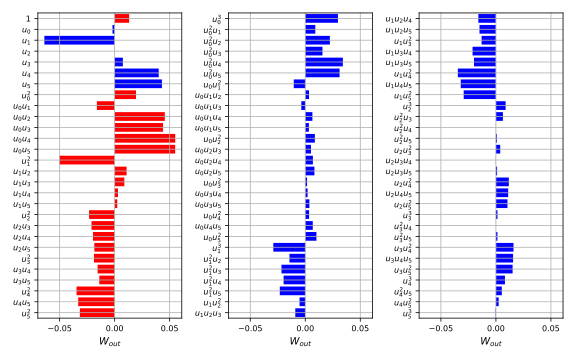
\includegraphics[width=\textwidth]{figures/nvar-predict-mackey-glass-wout}
  \caption{Weights in the matrix $W_\text{out}$ for the NVAR trained
    for Mackey-Glass system forecasting. Terms that break the
    inversion symmetry are in red. In labels, $u_i$ is shorthand for $u(t - \tau_i \Delta t)$. As the training signal does not
    reflect the inversion symmetry, the red terms are not trained to
    near zero as they are in \cref{fig:nvar-infer-lorenz-wout}.}
  \label{fig:nvar-predict-mackey-glass-wout}
\end{sidewaysfigure}

\section{Conclusion}

In this chapter, I have demonstrated the NVAR approach on two classic
RC problems: state inference and system forecasting. I show that
NVARs can solve these problems as well, or in some cases better, than
the RC approach, despite the simplicity of the NVAR method. At the
same time, I have resolved the remaining questions raised in
\cref{ch:nvar}: NVARs remain useful even with only a handful of
time-delay taps, and a simple extension of the nonlinear function
$\bm{g}_\text{n}$ to include higher-order monomial terms is sufficient
in many cases.

The Mackey-Glass forecasting task sits at the very edge of this simple
technique. It shows that a low number of time-delay taps remains
sufficient even in systems with long, built-in time delays, as long as the taps are chosen carefully. However,
it also demonstrates that a cubic nonlinearity is not sufficient to
reproduce the precise shape of the Mackey-Glass attractor. To move
forward with the NVAR technique, the nonlinear function
$\bm{g}_\text{n}$ will need to include much higher-order terms, and it
will need to do so without the exponential increase in training time
associated with adding more monomial terms to the output.

The Mackey-Glass system also demonstrates that symmetry matching is
not necessary or even desired in all cases when using an NVAR, if the
signal the NVAR is trained on never encounters that symmetry. In that
case, the NVAR will utilize terms that break the symmetry of the
underlying system in order to improve forecasting accuracy within the
volume of phase space that the training signal lies inside. This comes
with a trade-off: prediction outside this volume of phase space, such
as predicted fixed points, fails.

Even with the unresolved questions, I find the NVAR method is very
simple to implement and performs well. Due to its simplicity, I
recommend attempting to use an NVAR first in all cases where an RC is
considered.
